The goal of algebraic topology is to associate a collection of algebraic objects to a topological space.
Once this is done, abstract algebra can be employed to reason about global properties of the underlying space.

The two main ways of assigning invariants are homotopy and homology.
While homology is weaker than homotopy, it is more amenable to computation and is the direction we pursue.

\subsection{Mathematical Preliminaries}

Homology: properties of chains composed of oriented simplices
Elements of homology groups are cycles (chains with vanishing boundary).
Two k-cycles are homologous if they differ by the boundary of a (k+1)-chain.
Incidence matrix representation...

\subsubsection{Simplicial Complexes}

\paragraph{Simplex}




\paragraph{Chains, cycles and boundaries}

Boundary operator $\partial_{k}:C_{k}\rightarrow C_{k-1}$.
Action of boundary operator on a simplex $\sigma$ is defined as: 

\begin{equation}
\partial_{k}\sigma = \displaystyle\sum_{i}(-1)^{i}[v_{0},v_{1},...,\hat{v}_{i},...,v_{n}].
\end{equation}

A chain $C\in C_{k}$ is called a cycle if $\partial_{k}C=0$.
Chain with empty boundary.
Set of cycles forms a group.

Boundary operator defines a chain complex $C_{*}$:

\begin{equation}
\dots \overset{\partial_{n+1}}{\longrightarrow} C_n \overset{\partial_{n}}{\longrightarrow} C_{n-1} \overset{\partial_{n-1}}{\longrightarrow}  ... \overset{\partial_{2}}{\longrightarrow} C_n \overset{\partial_{1}}{\longrightarrow} C_{n-1} \overset{\partial_{0}}{\longrightarrow}  0
\end{equation}

Important property:

\begin{equation}
\partial_{k-1}\partial_{k} = 0 \forall k
\end{equation}

Intuitively, a boundary has no boundary.

$C$ is the set of 
The $k$-th cycle group is $Z_{k}=\ker \partial_{k}$.
$Z_{k}$ defines the set of all cycles of dimension $k$.
$B_{k}$ defines the set of all boundaries of dimension $k$.
That is, elements of $B_{k}$ serve as boundaries of $(k+1)$-chains.

TDA+PH: number and type of holes. which holes are essential and which are unimportant.

Basically get to the point where can define homology.
Chain complex.
Boundary operators
Work only over $\mod 2$ Homology (0,1) coefficients.
Torsion observed in the image patch data set, but no reason to think it is present biologial data sets we examine.

\begin{figure}
\centering
% \includegraphics[]{./fig/boundary_example.pdf}
\caption[]{}
\label{background:fig:boundary_example}
\end{figure}

\subsubsection{Homology}

Abelian groups generated by holes in the space.
Betti number is the rank of the homology group.

Simplical homology.
Abelian groups.
First homology group: abelianization of the fundamental gorup.
Quotient group

Recalling out definition of the boundary and cycle groups, define a quotient group

\begin{equation}
H_{k} = Z_{k} / B_{k} = \ker\partial_{k} / \im\partial_{k+1}
\end{equation}

Closed chains (cycles) up to boundary of higher dimensional cycles.
Elements are classes of homologous cycles.

\begin{figure}
\centering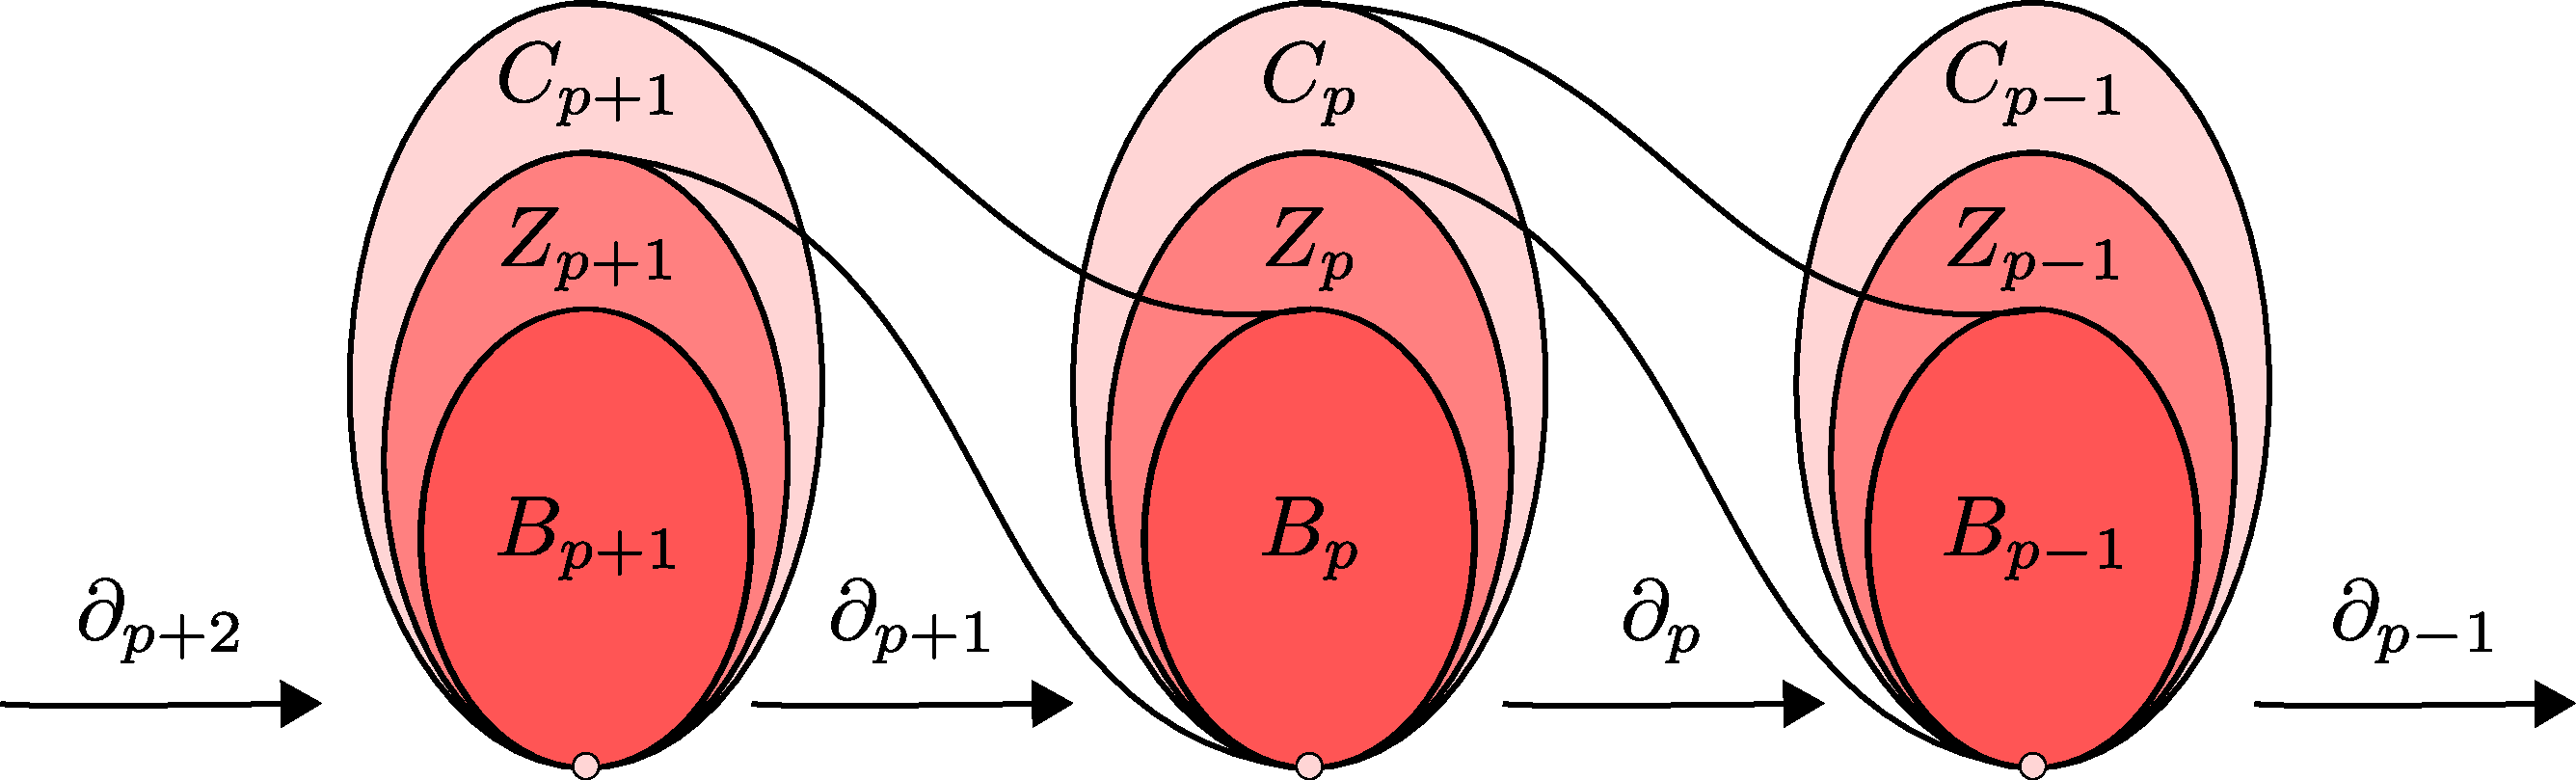
\includegraphics[width=\columnwidth]{./fig/FASY_chain_complexes.pdf}
\caption{Relationship between chain and cycle and homology. Adapted (``Adapted'') from Fasy.}
\label{fig:chain_complexes}
\end{figure}